\chapter{Problem statement}
\label{chap:problem-statement}

\section{Context}
\label{sec:context}

With the rise of the Internet of Things (IoT), fog computing has emerged as a new paradigm for processing data at the edge
of the network. Fog computing is an extension of cloud computing, as more devices become connected to the internet, the
amount of data generated by these devices increases. This data needs to be processed in real-time to provide insights and
make decisions. Cloud service providers and data centers are always looking for ways to optimize their resources and reduce
operational costs, particularly in terms of energy consumption. Fog computing can help by offloading tasks from the cloud to
the edge devices. They also need to satisfy the Quality of Service (QoS) requirements of the applications running on the
network, like low latency and high availability.

\section{Work environment}
\label{sec:work-environment}

This project was done within the office of the LAAS-CNRS laboratory in Toulouse, France. The laboratory is a research
institution that specializes in computer science, robotics, and automation. The following tools were used during the
project:

\begin{itemize}
  \item \textbf{Python}: a programming language that is widely used in scientific computing and machine learning.
  \item \textbf{GitHub}: a version control system that is widely used for software development.
  \item \textbf{QtFuzzyLite}: a software for fuzzy logic control with a graphical user interface.
  \item \textbf{Pyfuzzylite}: a Python library for fuzzy logic control.
  \item \textbf{Weka}: a collection of machine learning algorithms for data mining tasks.
  \item \LaTeX: a typesetting system that is widely used for scientific and technical documents.
  \item A personal computer running Windows 11 with a \textbf{Ryzen 7 6800H} processor and \textbf{32 GB} of RAM.
\end{itemize}

\section{Objective}
\label{sec:objective}

Our objective is to create a task scheduling algorithm for fog computing environments that considers multiple
parameters like energy consumption, latency, and resource utilization. The algorithm should be able to make decisions
about where to execute a task based on the current state of the system and the requirements of the task. It should be
able to adapt to changing conditions and make real-time decisions. The algorithm should be evaluated using simulations
and compared to existing algorithms to demonstrate its effectiveness.

\chapter{Internet of Things (IoT)}
\label{chap:iot}

The Internet of Things (IoT) is a network of interconnected devices that can communicate with each other and exchange
data. These devices can be anything from smartphones and laptops to sensors and actuators. The IoT is a rapidly growing
field with many applications in various industries like healthcare, agriculture, transportation, and manufacturing.
The goal of the IoT is to make our lives easier by automating tasks and providing real-time information.

It is made possible by advances in wireless communication, sensor technology, and cloud computing. These technologies
allow devices to connect to the internet and share data with each other and the cloud. The IoT has many benefits like
improved efficiency, reduced costs, and increased safety. However, it also has some challenges like security, privacy,
and interoperability.

IoT is a key enabler of fog computing, as such it is important to understand its history, architecture, and applications.
This chapter will provide an overview of the IoT and its role in fog computing.

\section{History}
\label{sec:iot-history}

The concept and the term "Internet of Things" can be traced back to the 1985 during a speech by Peter T. Lewis to the
Congressional Black Caucus Foundation.\cite{chetansharma-2016} He said: "The Internet of Things, or IoT, is the
integration of people, processes and technology with connectable devices and sensors to enable remote monitoring,
status, manipulation and evaluation of trends of such devices." The term was later popularized by Kevin Ashton in
1999.\cite{ashton-2009}

The first internet-connected (previously known as ARPANET) device was a Coca-Cola vending machine at Carnegie Mellon
University in 1982,\cite{cscmuedu} it was able to report its inventory and temperature to the network. Since then,
the IoT has grown rapidly with the advent of wireless communication, sensor technology, and cloud computing.

Cisco Systems estimated that the number of internet-connected devices exceeded the number of people on Earth between
2008 and 2009,\cite{evans-2011} marking the beginning of the IoT era. Today, there are billions of IoT devices around
the world, and the number will continue to grow as more devices become connected.

\section{Architecture}
\label{sec:iot-architecture}

The IoT architecture consists of three layers: the perception layer, the network layer, and the application layer.
\begin{itemize}
  \item The perception layer is where the devices are located, it includes sensors, actuators, and other devices that
        collect data and interact with the physical world.
  \item The network layer is where the devices communicate with each other and the cloud, it includes wireless
        communication technologies like Wi-Fi, Bluetooth, and Zigbee.
  \item The application layer is where the data is processed and analyzed, it includes cloud computing services like
        Amazon Web Services (AWS), Microsoft Azure, and Google Cloud Platform.
\end{itemize}

The IoT architecture is designed to be scalable, flexible, and secure. It allows devices to connect to the internet and
share data with each other and the cloud. This enables new applications and services that were not possible before. The
IoT architecture is still evolving with new technologies like edge computing and fog computing. These technologies bring
the cloud closer to the devices and reduce latency and bandwidth requirements.

\section{Applications}
\label{sec:iot-applications}

\subsection{Home automation}
\label{subsec:iot-home-automation}

One of the most popular applications of the IoT is home automation, it allows homeowners to control many aspects of their
home like lighting, heating, and security. Smart devices like thermostats, light bulbs, and cameras can be connected to
the internet and controlled remotely using a smartphone or voice assistant.

Home automation can help homeowners save energy, improve security, and make their lives more convenient. It is also a
growing market with many companies offering smart home products and services, like Google Home, Amazon Echo, and Apple
HomeKit. Non-proprietary solutions are also available, like Home Assistant, OpenHAB, and Domoticz.

\subsection{Healthcare}
\label{subsec:iot-healthcare}

IoT has many applications in healthcare, it can be used to monitor patients, track medications, and manage chronic diseases.
Wearable devices like smartwatches and fitness trackers can collect data on a patient's heart rate, blood pressure, and
activity level. This data can be sent to a healthcare provider for analysis and diagnosis. The IoT can also be used to monitor
patients in hospitals and nursing homes, it can alert healthcare providers if a patient's condition changes. The IoT can help
improve patient outcomes, reduce costs, and increase access to care.

However, it also raises concerns about privacy, security, and data ownership. The Health Insurance Portability and Accountability
Act (HIPAA)[\href{https://www.hhs.gov/hipaa/for-professionals/privacy/index.html}{HIPAA privacy rule}] in the United States
and the General Data Protection Regulation
(GDPR)[\href{https://www.cnil.fr/fr/reglement-europeen-protection-donnees/chapitre1#Article4}{article 4-15}] in the European
Union are two regulations that govern the use of healthcare data.

\subsection{Energy management}
\label{subsec:iot-energy-management}

Homeowners can monitor and control their energy usage using with many IoT devices, this principle can be extended to a larger
scale with smart grids. Smart grids are electrical grids that use IoT devices to monitor and control the flow of electricity.
They can help utilities reduce costs, improve reliability, and increase efficiency. They can also help reduce greenhouse gas
emissions and promote renewable energy sources. It is a growing field with many companies offering smart grid products and
services, like Siemens, ABB, and Schneider Electric.

\begin{figure}[H]
  \centering
  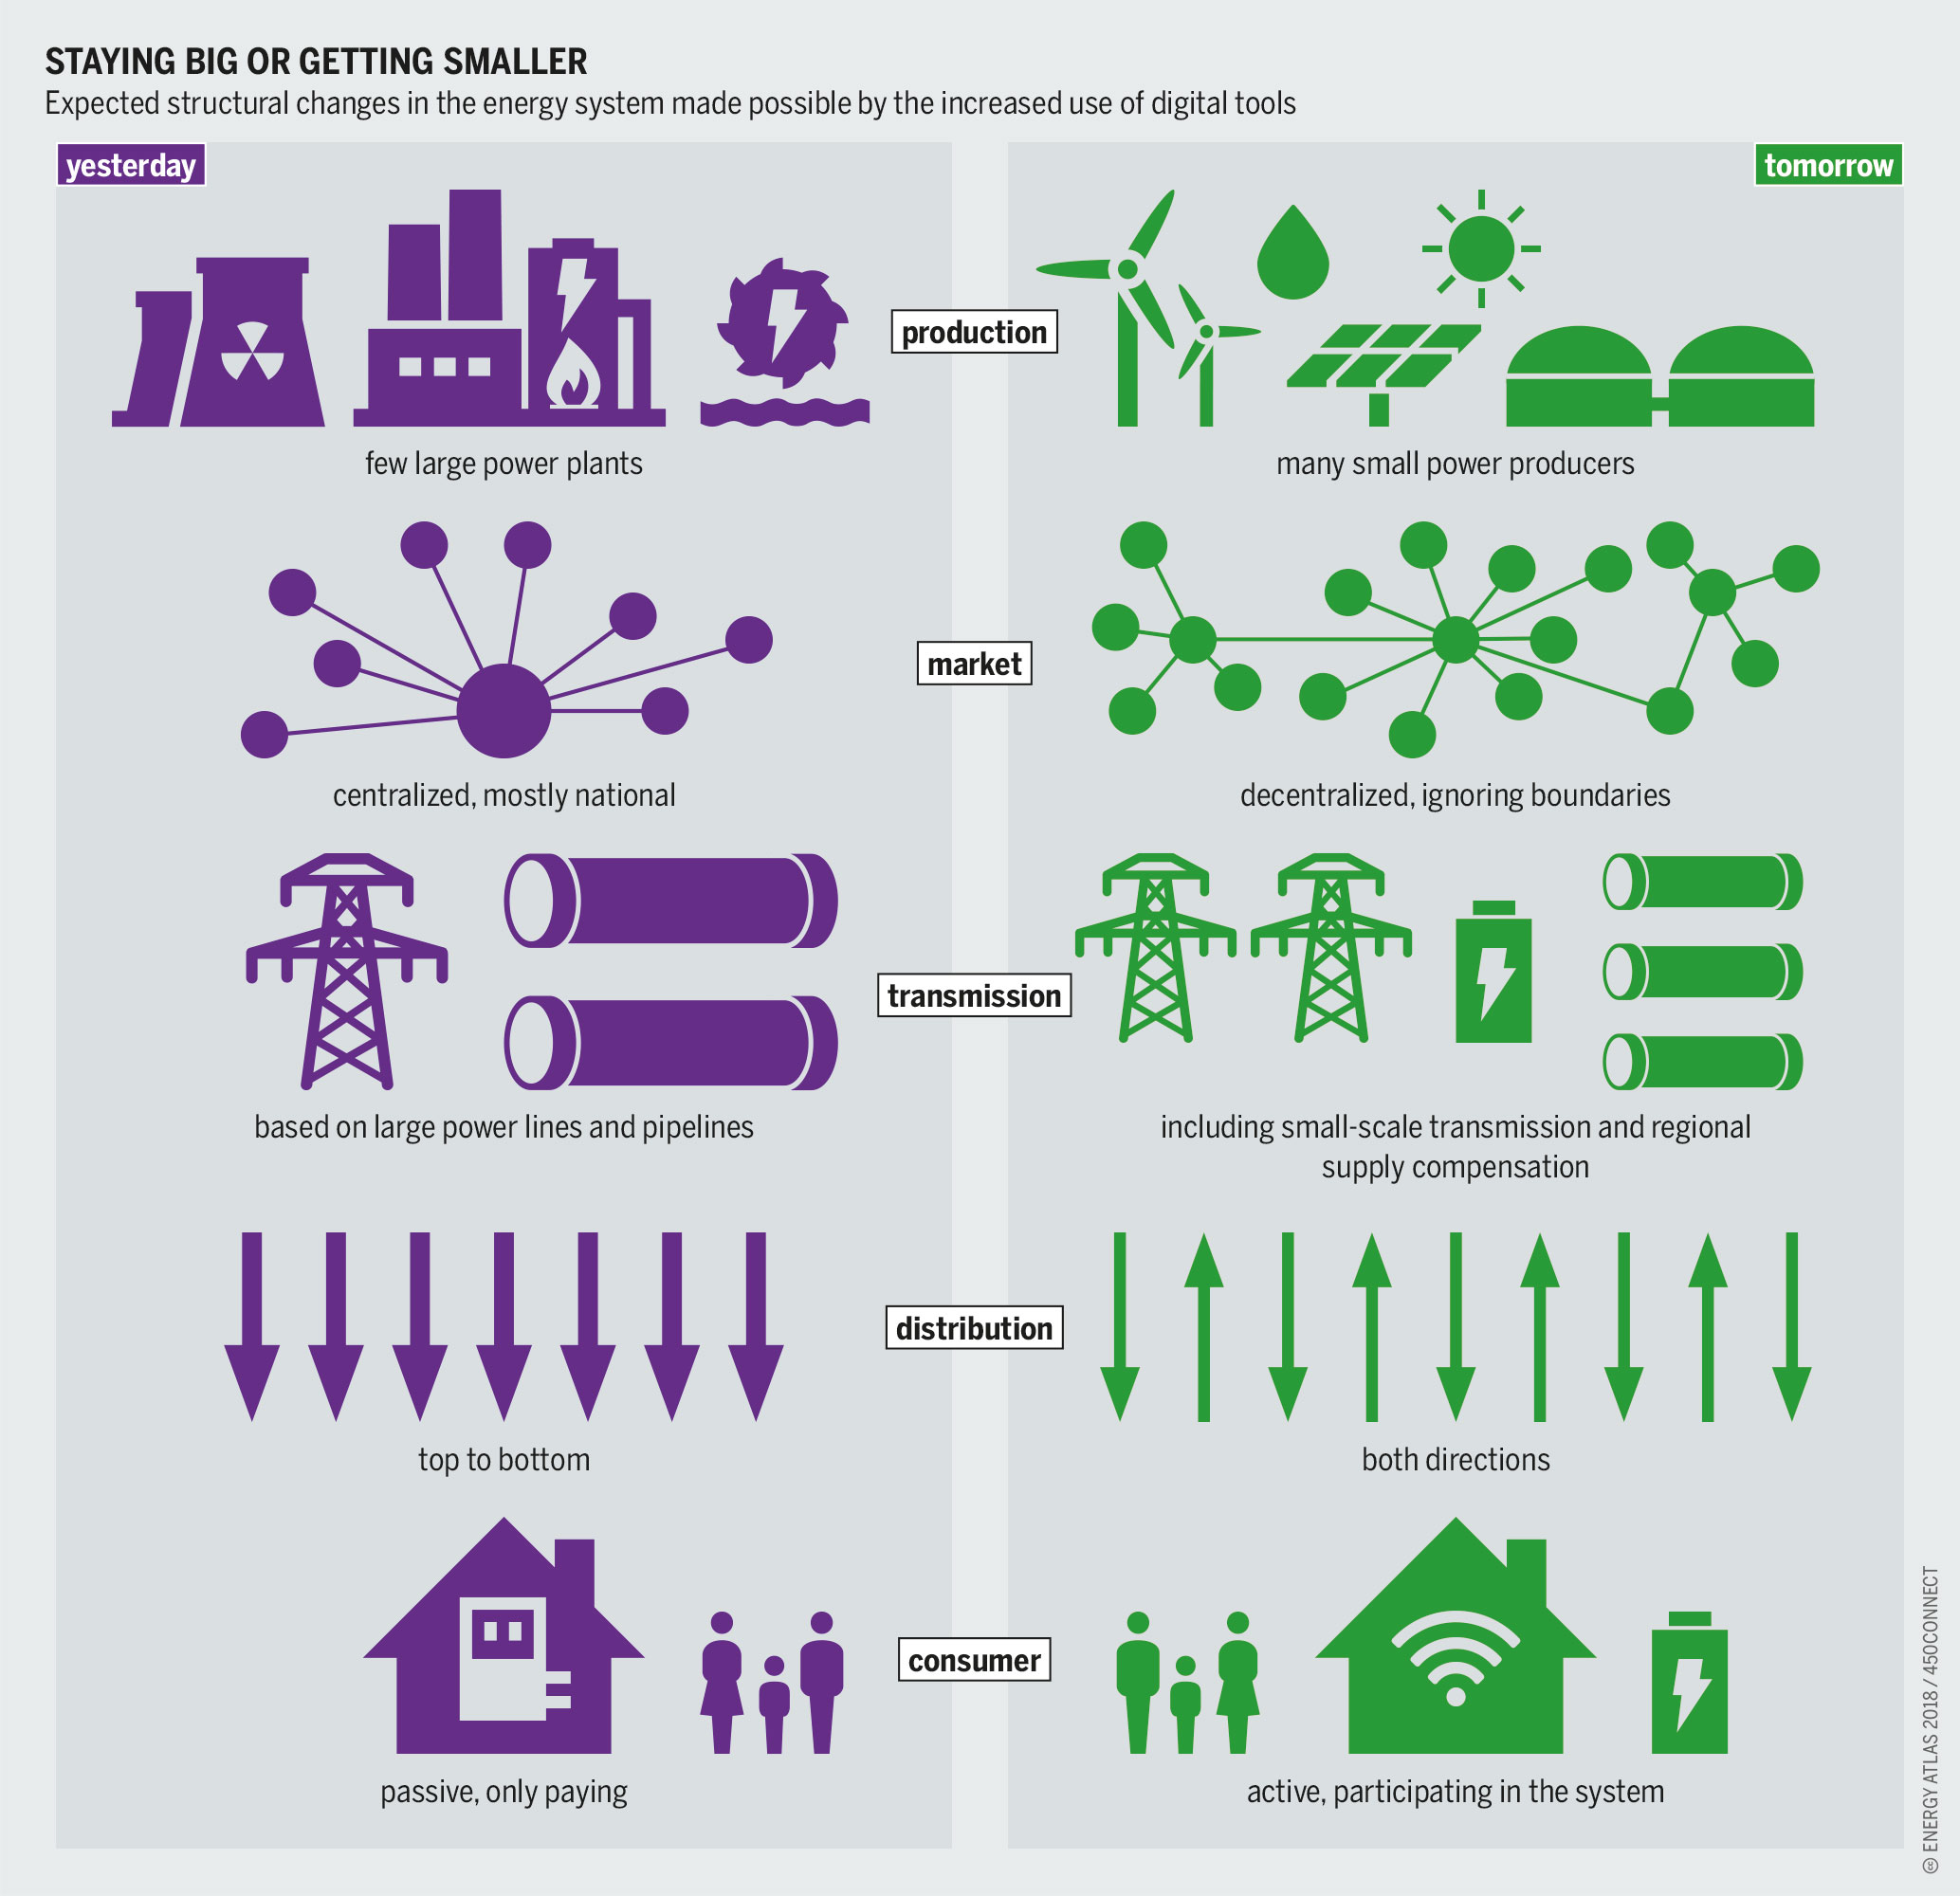
\includegraphics[width=0.80\textwidth]{../images/smart-grid.jpg}
  \caption{Characteristics of a traditional system (left) versus the smart grid (right)~\cite{bartz-stockmar-2018}}
  \label{fig:smart-grid}
\end{figure}

\chapter{FOG computing}
\label{chap:fog}

FOG computing was introduced by Cisco in 2012 as a way to extend cloud computing to the edge of the network. The goal
of FOG computing is to bring the cloud closer to the end-users, this is done by placing the cloud's resources at the
edge of the network thanks to a wider geographical distribution.

\section{Concept}
\label{sec:fog-concept}

FOG computing is a virtualized and decentralized computing platform that acts as an intermediary between the cloud and
the edge devices. The word "fog" is used to describe the cloud-like properties being closer to the "ground", the ground
being the edge devices. Many of these devices will generate a huge amount or raw data that needs to be processed in real
time, this is where FOG computing comes in. Instead of sending all the data to the cloud for processing, the data is
processed on FOG nodes. The nodes can be anything from resource-rich servers to resource-constrained devices like
gateways, routers or other end devices.

It is designed to reduce latency, provide computing resources, storage and network services to the edge devices. It also
provides location awareness, mobility support, and real-time data processing. FOG computing is ideal for applications that
require real-time processing, like autonomous vehicles, industrial automation, and augmented reality.

However, FOG computing is not to be confused with edge computing, while they share some similarities, they are not the
same. Edge computing is a subset of FOG computing, the processing is done at the edge of the network, while FOG computing
allows the processing to be done anywhere between the edge and the cloud.

\section{Architecture}
\label{sec:fog-architecture}

The architecture of a FOG network is shown in figure \ref{fig:fog-architecture}. It consists of three layers:
\begin{itemize}
  \item The edge layer is where the end devices are located, it includes sensors, actuators, and other devices that
        generate data.
  \item The FOG layer is where the FOG nodes are located, it includes servers, gateways, and other devices that
        process data.
  \item The cloud layer is where the cloud data centers are located, it includes servers, storage, and network
        services that store and process data.
\end{itemize}

\begin{figure}[H]
  \centering
  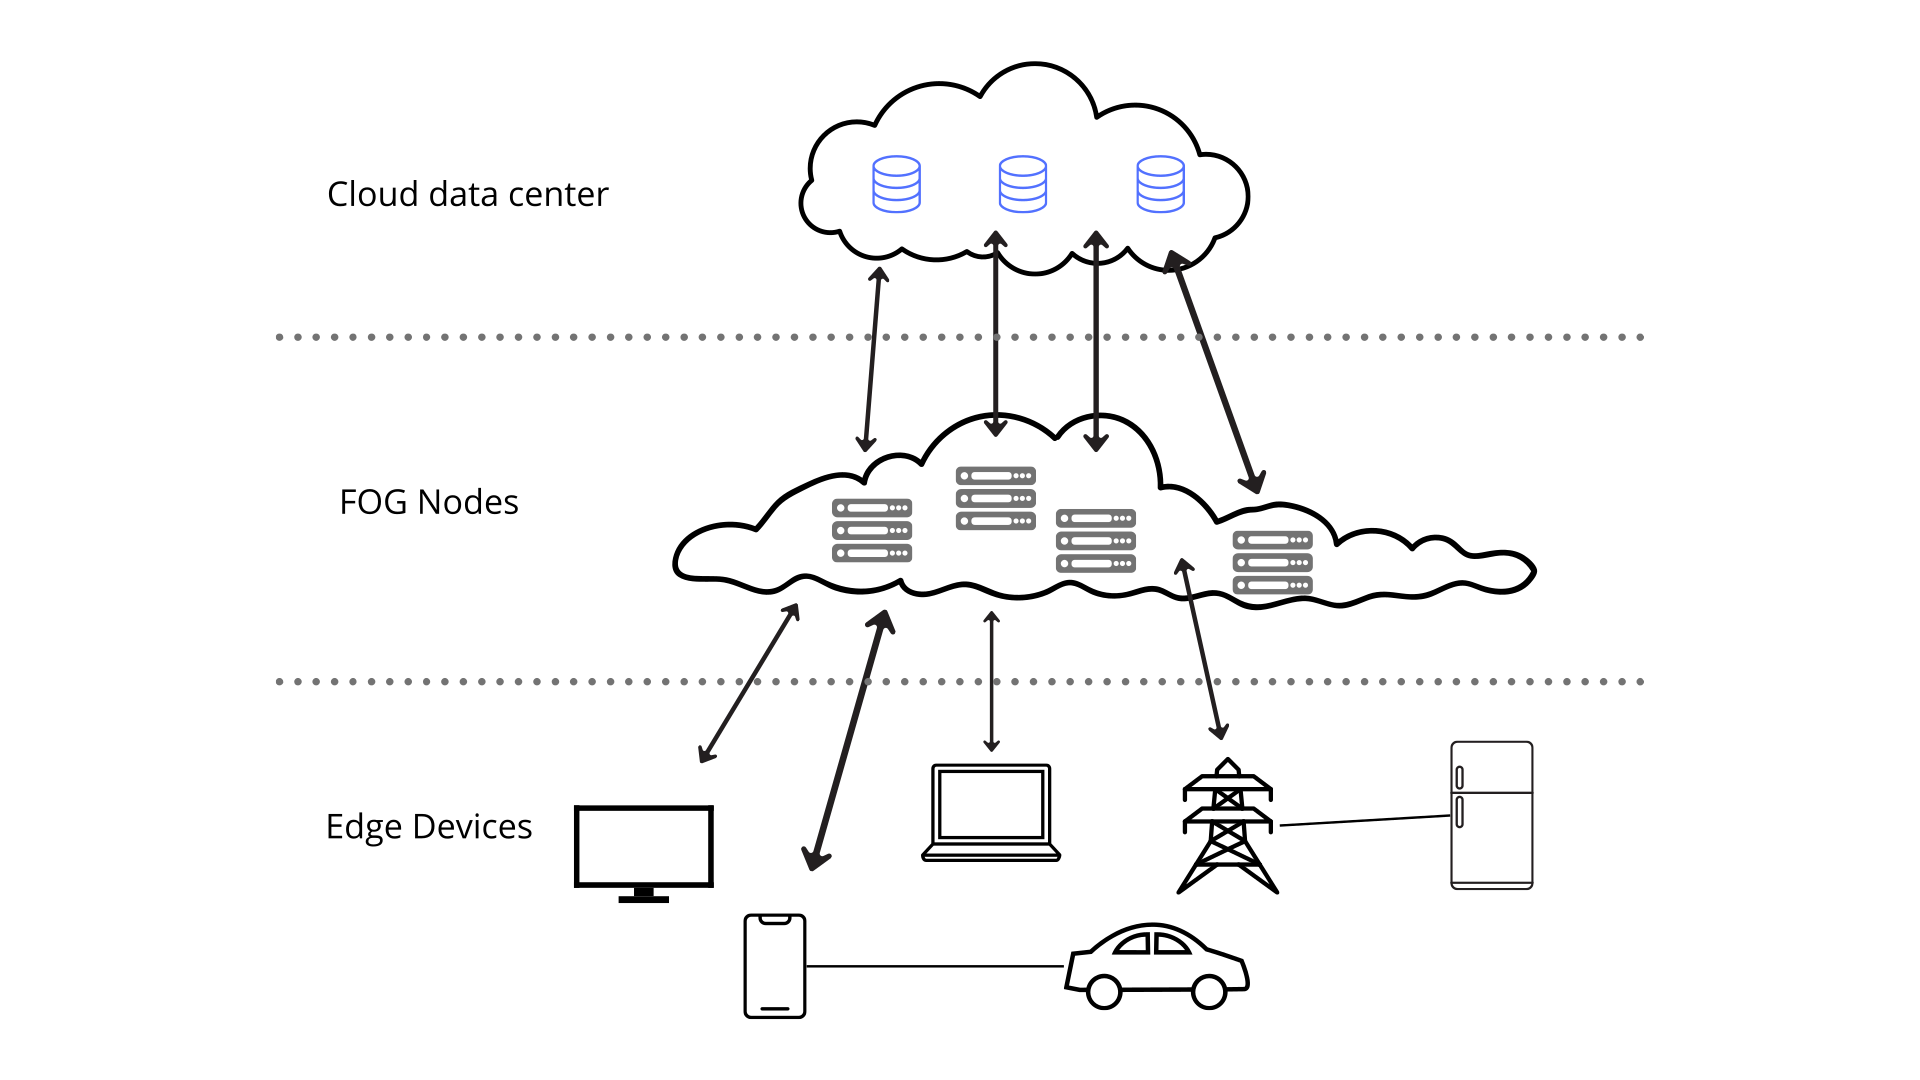
\includegraphics[width=0.70\textwidth]{../images/FOG_network_ink.png}
  \caption{FOG computing architecture.}
  \label{fig:fog-architecture}
\end{figure}

\section{Challenges}
\label{sec:fog-challenges}

While FOG networking has many benefits, it also has some challenges. Some of these challenges are inherited from cloud
computing, while others are unique to FOG computing. We will a few of these challenges in the following sections.

\subsection{Security and privacy}
\label{subsec:fog-security}

As the number of connected devices and fog nodes increases, so does the complexity of the network. This complexity makes
it difficult to ensure date security and privacy. The data generated by the end devices can be sensitive and needs to be
protected from unauthorized access. Also, as some fog nodes are making use of virtualized infrastructure, they
introduce vulnerabilities in hypervisors and virtual machines.

\subsection{Energy efficiency}
\label{subsec:fog-energy}

FOG computing requires many devices to be connected to the network, this can lead to increased energy consumption. The
amount of nodes and servers needed to process the data can be significant, this can lead to increased cooling and power
costs. To address this issue, fog nodes can be equipped with energy-efficient hardware and software, like low-power
processors and energy-aware scheduling algorithms.

\subsection{Quality of service (QoS)}

FOG computing requires real-time processing of data, this can be challenging as the network conditions can change rapidly.
It requires a reliable and low-latency network to ensure that the data is processed in a timely manner. The bandwidth
and latency requirements need to be met to ensure that the data is processed correctly. To address this issue, fog nodes
can be equipped with QoS mechanisms that prioritize traffic based on its importance.

\chapter{Offloading using Fuzzy logic}
\label{chap:fuzzy}

We decided to use fuzzy logic to implement a decision engine for offloading tasks in a fog computing environment. We chose
this approach because fuzzy logic is well-suited for making decisions based on imprecise and uncertain data, which is
common in fog computing environments.  It is also able to handle multiple inputs and outputs, which is important in a
complex system like fog computing.

\section{Explaining fuzzy logic}
\label{sec:fuzzy-explanation}

Introduced in 1965 by Lotfi Zadeh,\cite{zadeh-1965} fuzzy logic is based on a "degree of truth" instead of a finite
value, usually 0 or 1, it aims to represent the vagueness of human language and thought. Fuzzy systems are the means
to implement fuzzy logic, they are two types of fuzzy systems: Mamdani and Sugeno, both are similar but differ in the
way the output is determined. The most common one Mamdani and it's the one we will be using in this project. The
Mamdani fuzzy system follows three steps:

\begin{itemize}
  \item The inputs are fuzzified into fuzzy membership functions,
  \item a set of rules are applied to the fuzzy inputs to determine the fuzzy output,
  \item the fuzzy output is defuzzified to get a crisp value.
\end{itemize}

While Sugeno includes the defuzzification step in the rule evaluation step, this system works well with optimization
algorithms and is more computationally efficient than the Mamdani system. But for this project we will be using the
Mamdani system.

\subsection{Fuzzification}
\label{subsec:fuzzy-fuzzification}

Fuzzification is the process of converting a crisp value into a fuzzy value, this is done by assigning a membership
function to the input value. The membership function is a curve that defines how much the input value belongs to a
certain fuzzy set. The most common fuzzy sets are the triangular and trapezoidal functions, they are defined by three
or four parameters respectively. The triangular function is defined by the parameters $a$, $b$ and $c$ and is given by:

\begin{equation}
  \mu(x) = \begin{cases}
    0                   & \text{if } x \leq a,        \\
    \frac{x - a}{b - a} & \text{if } a \leq x \leq b, \\
    \frac{c - x}{c - b} & \text{if } b \leq x \leq c, \\
    0                   & \text{if } x \geq c.
  \end{cases}
\end{equation}

The trapezoidal function is defined by the parameters $a$, $b$, $c$ and $d$ and is given by:

\begin{equation}
  \mu(x) = \begin{cases}
    0                   & \text{if } x \leq a,        \\
    \frac{x - a}{b - a} & \text{if } a \leq x \leq b, \\
    1                   & \text{if } b \leq x \leq c, \\
    \frac{d - x}{d - c} & \text{if } c \leq x \leq d, \\
    0                   & \text{if } x \geq d.
  \end{cases}
\end{equation}

\subsection{Rule evaluation}
\label{subsec:fuzzy-rule-evaluation}

The rule evaluation is the process of determining the fuzzy output based on the fuzzy inputs and a set of rules. The
rules are defined by two parts: the "if" or antecedent part and the "then" or consequent part. The antecedent part
deals with inputs, it can either be a single input or a combination of inputs, the combination can be done using the
logical operators "and" and "or". The consequent part deals with the output. In the context of this project, the rules
are usually of the form "if Bandwidth is low then processing is local". The rules are generally defined by the user
and are based on their knowledge of the system.

\subsection{Aggregation}
\label{subsec:fuzzy-aggregation}

The aggregation is the process of combining the fuzzy outputs from the rules to get a single fuzzy output. This process
relies on T-conorms, and must satisfy the following properties:

\begin{itemize}
  \item Commutativity: $x * y = y * x$,
  \item Associativity: $x * (y * z) = (x * y) * z$,
  \item Monotony: $x \leq y \implies x * z \leq y * z$,
  \item Neutrality of 0: $x * 0 = x$ for $x \in [0, 1]$.
\end{itemize}

They are also \textit{positive reinforcement} operators:

\begin{equation}
  f(x_1, \cdots, x_n) \leq max[x_i] \forall x_i \geq 0.5
\end{equation}

As opposed to T-norms which are \textit{negative reinforcement} operators:

\begin{equation}
  f(x_1, \cdots, x_n) \geq min[x_i] \forall x_i \leq 0.5
\end{equation}

The most common T-conorms are the maximum, the probabilistic sum and the bounded sum. They are defined as follows:

\begin{minipage}{0.9624\textwidth}
  \begin{equation}
    \text{Maximum: } x \oplus y = \max(x, y)
  \end{equation}
  \begin{equation}
    \text{Probabilistic sum: } x \oplus y = x + y - x \cdot y
  \end{equation}
  \begin{equation}
    \text{Bounded sum: } x \oplus y = \min(x + y, 1)
  \end{equation}
\end{minipage}

\subsection{Defuzzification}
\label{subsec:fuzzy-defuzzification}

Defuzzification is the process of converting a fuzzy output into a crisp value, there are several methods to do this,
the most common one is the centroid method. The centroid method calculates the center of mass of the fuzzy output, this
is done by taking the weighted average of the output values. The weighted average is calculated by taking the sum of
the product of the output value and its membership value divided by the sum of the membership values. The formula for
the centroid method is given by:

\begin{equation}
  y = \frac{\sum_{i} \mu_i \cdot y_i}{\sum_{i} \mu_i}
\end{equation}

Where $y$ is the crisp output, $\mu_i$ is the membership value of the output value $y_i$. The centroid method is the
most common method because it is simple and easy to implement. However, it is not always the best method, other methods
like the mean of maximum and the largest of maximum can be used depending on the application.

\section{Fuzzy system for offloading}
\label{sec:fuzzy-offloading}

\subsection{Setting up the engine}
\label{subsec:fuzzy-setup}


\begin{table}[H]
  \centering
  \begin{tabular}{|c|c|c|c|c|}
    \hline
    Name                & Range    & Fuzzy set & Membership function & Parameters         \\
    \hline
    Bandwidth           & [0, 100] & bw_low    & trapezoidal         & 0, 20, 30, 40      \\
    (in Mbps)           &          & bw_med    & trapezoidal         & 35, 45, 60, 70     \\
                        &          & bw_high   & trapezoidal         & 65, 75, 90, 100    \\
    \hline
    Data size           & [0, 600] & data_low  & trapezoidal         & 0, 0, 230, 360     \\
    (in KB)             &          & data_med  & trapezoidal         & 250, 350, 470, 590 \\
                        &          & data_high & trapezoidal         & 450, 540, 600, 600 \\
    \hline
    Residual battery    & [0, 100] & bat_low   & trapezoidal         & 0, 0, 25, 35       \\
    charge (in \%)      &          & bat_med   & trapezoidal         & 25, 40, 60, 75     \\
                        &          & bat_high  & trapezoidal         & 60, 75, 100, 100   \\
    \hline
    Load                & [0, 100] & load_low  & trapezoidal         & 0, 0, 25, 40       \\
    (in \%)             &          & load_med  & trapezoidal         & 35, 45, 60, 70     \\
                        &          & load_high & trapezoidal         & 65, 80, 100, 100   \\
    \hline
    Memory              & [0, 100] & mem_low   & trapezoidal         & 0, 0, 25, 40       \\
    (in \%)             &          & mem_med   & trapezoidal         & 35, 45, 60, 70     \\
                        &          & mem_high  & trapezoidal         & 65, 80, 100, 100   \\
    \hline
    Virtual machines    & [0, 50]  & vm_low    & trapezoidal         & 0, 0, 15, 20       \\
    available           &          & vm_med    & trapezoidal         & 15, 22, 37, 40     \\
                        &          & vm_high   & trapezoidal         & 30, 35, 50, 50     \\
    \hline
    Number              & [0, 100] & user_low  & trapezoidal         & 0, 0, 25, 40       \\
    of concurrent users &          & user_med  & trapezoidal         & 30, 40, 60, 70     \\
                        &          & user_high & trapezoidal         & 60, 75, 100, 100   \\
    \hline
  \end{tabular}
  \caption{Input variables for the fuzzy engine.}
  \label{tab:fuzzy-input}
\end{table}

To demonstrate the use of fuzzy logic in offloading, we wrote two simple programs in Python. The goal was to recreate
the experiment done by Hari et al.\cite{Hari-et-al-2018} The first program uses the \textit{pyfuzzylite}\cite{fuzzylite}
library to implement a fuzzy engine with all the variables and rules needed to determine the offloading decision. The
second program uses the NumPy library to generate random values for the inputs and then uses the fuzzy engine to determine
the offloading decision (remote execution or local execution, remote execution means offloading the task to the cloud or
a fog node). The fuzzy engine is defined by the variables shown in table \ref{tab:fuzzy-input} and \ref{tab:fuzzy-output}.

\begin{table}[H]
  \centering
  \begin{tabular}{|c|c|c|c|c|}
    \hline
    Name                & Range    & Fuzzy set & Membership function & Parameters      \\
    \hline
    Offloading decision & [0, 100] & local     & trapezoidal         & 0, 12, 24, 48   \\
                        &          & remote    & trapezoidal         & 36, 60, 72, 100 \\
    \hline
  \end{tabular}
  \caption{Output variable for the fuzzy engine.}
  \label{tab:fuzzy-output}
\end{table}

The original paper by Hari et al. did not provide all the rules used, so we had to come up with our own rules. We
established them based on our understanding of the system and the variables. Unlike the original paper, where the
rules only combined the bandwidth with one other variable, we decided to combine the bandwidth with all the relevant
variables. The rules are shown in table \ref{tab:fuzzy-rules}.

\begin{table}[H]
  \centering
  \resizebox{\textwidth}{!}{%
    \begin{tabular}{|l|l|}
      \hline
         & Rules                                                                                                  \\
      \hline
      R1 & IF Bandwidth is bw_low                                                                                 \\
         & THEN Processing local_processing                                                                       \\
      \hline
      R2 & IF Bandwidth is not bw_low and Datasize is not data_low                                                \\
         & THEN Processing is remote_processing                                                                   \\
      \hline
      R3 & IF Bandwidth is not bw_low and Datasize is data_low and (Load is load_high or Memory is mem_low)       \\
         & THEN Processing is remote_processing                                                                   \\
      \hline
      R4 & IF Bandwidth is not bw_low and Datasize is data_low and (NB_concurrent_users is user_low or Memory is
      mem_low)                                                                                                    \\
         & THEN Processing is remote_processing                                                                   \\
      \hline
      R5 & IF Bandwidth is not bw_low and Datasize is data_low and NB_concurrent_users is not user_low and Memory
      is not mem_low and Load is load_low                                                                         \\
         & THEN Processing is local_processing                                                                    \\
      \hline
      R6 & IF Bandwidth is not bw_low and Datasize is data_low and NB_concurrent_users is not user_low and Memory
      is not mem_low and Load is not load_low                                                                     \\
         & THEN Processing is remote_processing                                                                   \\
      \hline
    \end{tabular}}
  \caption{Rules for the fuzzy engine.}
  \label{tab:fuzzy-rules}
\end{table}

From these rules we can see that two variables have no impact on the offloading decision, the residual battery charge
and the number of virtual machines available. So we decided to remove them from the fuzzy engine.

\subsection{Mean 3\texorpdfstring{$\Pi$}{Pi} aggregation operator (M3\texorpdfstring{$\Pi$}{Pi})}

The standard 3$\Pi$ operator was introduced by Yager and Rybalov \cite{yager-rybalov-1998} in 1988, it is a
generalization of the probabilistic sum. The 3$\Pi$ operator is defined by the following formula:

\begin{equation}
  \Pi(x_1, \cdots, x_n) = \frac{\Pi_{j=1}^n x_j}{\Pi_{j=1}^n x_j + \Pi_{j=1}^n (1 - x_j)}
\end{equation}

Unlike T-norms and T-conorms, the 3$\Pi$ operator is \textit{full reinforced} which means that it satisfies the
properties of both positive and negative reinforcement operators.

We decided to implement a M3$\Pi$ aggregation operator which is derived from the 3$\Pi$ operator, it is defined
by the following formula:

\begin{equation}
  M3\Pi(x_1, \cdots, x_n) = \frac{\Pi_{j=1}^n (x_j)^{(1/n)}}{\Pi_{j=1}^n (x_j)^{(1/n)} + \Pi_{j=1}^n (1 - x_j)^{(1/n)}}
\end{equation}

According to \cite{doncescu-et-al-2007}, if we consider the standard arithmetic mean $\frac{1}{n}\sum_{j=1}^{n}x_j$, then: \\
$\forall j \in 1, \cdots, n$, we have:

\begin{equation}
  M3\Pi(x_1, \cdots, x_n) \geq \frac{1}{n}\sum_{j=1}^{n}x_j, \text{ if } x_j \geq 0.5
\end{equation}

and:

\begin{equation}
  M3\Pi(x_1, \cdots, x_n) \leq \frac{1}{n}\sum_{j=1}^{n}x_j, \text{ if } x_j \leq 0.5
\end{equation}

The authors of \cite{doncescu-et-al-2007} named this property \textit{mean reinforcement}.

The goal was to improve the decision-making process. However, we were unable to implement the M3$\Pi$ operator as it
would require to modify a large part of the \textit{pyfuzzylite} library. The library is relatively complex and the
intricacies of the implementation were beyond our expertise. We decided to shift our focus towards other parts of
the project.

\subsection{Partial results}
\label{subsec:fuzzy-results}

Despite the absence of the M3$\Pi$ operator, we still ran the fuzzy engine with three different aggregation operators:
maximum, probabilistic sum and bounded sum. Samples of the results are shown in tables \ref{tab:fuzzy-results-max},
\ref{tab:fuzzy-results-prob} and \ref{tab:fuzzy-results-bounded}.

\begin{table}[H]
  \centering
  \resizebox{\textwidth}{!}{%
    \begin{tabular}{|l|l|l|l|l|l|l|l|l|}
      \hline
      Bandwidth & Data size & Number of        & Memory & Load & Crisp  & Fuzzy output                                     \\
                &           & concurrent users &        &      & output &                                                  \\
      \hline
      30        & 180       & 42               & 38     & 66   & 21.575 & 1.000/local_processing + 0.000/remote_processing \\
      77        & 462       & 44               & 96     & 8    & 67.539 & 0.000/local_processing + 1.000/remote_processing \\
      3         & 21        & 45               & 75     & 50   & 60.732 & 0.150/local_processing + 0.850/remote_processing \\
      38        & 229       & 51               & 31     & 66   & 57.565 & 0.200/local_processing + 0.600/remote_processing \\
      50        & 302       & 17               & 96     & 92   & 68.116 & 0.000/local_processing + 0.554/remote_processing \\
      \hline
    \end{tabular}}
  \caption{Sample results from the fuzzy engine with the Maximum aggregation operator.}
  \label{tab:fuzzy-results-max}

  \bigskip

  \centering
  \resizebox{\textwidth}{!}{%
    \begin{tabular}{|l|l|l|l|l|l|l|l|l|}
      \hline
      Bandwidth & Data size & Number of        & Memory & Load & Crisp  & Fuzzy output                                     \\
                &           & concurrent users &        &      & output &                                                  \\
      \hline
      30        & 180       & 42               & 38     & 66   & 21.575 & 1.000/local_processing + 0.000/remote_processing \\
      77        & 462       & 44               & 96     & 8    & 67.539 & 0.000/local_processing + 1.000/remote_processing \\
      3         & 21        & 45               & 75     & 50   & 60.443 & 0.150/local_processing + 0.850/remote_processing \\
      38        & 229       & 51               & 31     & 66   & 61.27  & 0.200/local_processing + 0.904/remote_processing \\
      50        & 302       & 17               & 96     & 92   & 68.314 & 0.000/local_processing + 0.863/remote_processing \\
      \hline
    \end{tabular}}
  \caption{Sample results from the fuzzy engine with the Probabilistic sum
    aggregation operator (note: the library calls it Algebraic sum).}
  \label{tab:fuzzy-results-prob}

  \bigskip

  \centering
  \resizebox{\textwidth}{!}{%
    \begin{tabular}{|l|l|l|l|l|l|l|l|l|}
      \hline
      Bandwidth & Data size & Number of        & Memory & Load & Crisp  & Fuzzy output                                     \\
                &           & concurrent users &        &      & output &                                                  \\
      \hline
      30        & 180       & 42               & 38     & 66   & 21.575 & 1.000/local_processing + 0.000/remote_processing \\
      77        & 462       & 44               & 96     & 8    & 67.539 & 0.000/local_processing + 1.000/remote_processing \\
      3         & 21        & 45               & 75     & 50   & 60.275 & 0.150/local_processing + 0.850/remote_processing \\
      38        & 229       & 51               & 31     & 66   & 61.855 & 0.200/local_processing + 1.000/remote_processing \\
      50        & 302       & 17               & 96     & 92   & 67.903 & 0.000/local_processing + 1.000/remote_processing \\
      \hline
    \end{tabular}}
  \caption{Sample results from the fuzzy engine with the Bounded sum aggregation operator.}
  \label{tab:fuzzy-results-bounded}
\end{table}

For the rest of the project, we will use the Maximum aggregation operator as it gave the best results. We will also focus
on improving the decision-making process by using a decision tree.

\chapter{Decision trees}
\label{chap:decision-trees}

In an attempt to improve the offloading decision-making process, we decided to use the Weka\cite{weka} software to create
a decision tree. We will use the J48 algorithm which is a Java implementation of the C4.5 algorithm. The goal is to was to
improve upon the decision-making process of the fuzzy engine.

\section{The Weka software}
\label{sec:weka}

Weka is a collection of machine learning algorithms for data processing and predictive modeling. It is written in Java and
is distributed under the GNU General Public License. The software is designed to be user-friendly and easy to use, thanks
to its graphical user interface. It is widely used in academia and industry for data mining, machine learning, and predictive
analytics. Weka provides a wide range of algorithms for classification, regression, clustering, etc. The software also
provides access to SQL databases with Java Database Connectivity (JDBC) and can also accept multiple data formats like
ARFF, CSV, C4.5, etc.

\begin{figure}[H]
  \centering
  \begin{minipage}[t]{0.48\textwidth}
    \centering
    
\includegraphics[width=1\linewidth]{../images/Weka_logo.png}
    \caption{Weka logo.}
    \label{fig:waka-logo}
  \end{minipage}\hfill
  \begin{minipage}[t]{0.48\textwidth}
    \centering
    
\includegraphics[width=0.5\linewidth]{../images/weka-icon.png}
    \caption{Weka software icon.}
    \label{fig:waka-icon}
  \end{minipage}
\end{figure}

\subsection{The J48 algorithm}
\label{subsec:j48}

The J48 algorithm is a decision tree algorithm, it allows the creation of a decision tree from a set of training data. The
algorithm works by recursively splitting the data into subsets based on the values of the input variables. The goal is to
create a tree that can predict the value of the output variable based on the input variables. The algorithm uses the
information gain to determine the best split at each node, the information gain is a measure of the reduction in entropy.

The training data is a set of already classified data, it contains the values of the input variables and the corresponding
value of the output variable and the class it belongs to. The algorithm uses this data to build the decision tree, at each
node, it selects the attribute that split the data into the best subsets. The process is repeated until all the data is
classified. The decision tree can then be used to predict the value of the output variable for new data.

Decision trees are used to represent the decision-making process in a graphical form, they are easy to understand and
interpret. They can also be used to identify the most important variables in the data and to detect patterns and
relationships between the variables.

\subsection{The decision tree}
\label{subsubsec:decision-tree}

The resulting decision tree is composed of nodes, leaves and branches:
\begin{itemize}
  \item The nodes represent the attributes where the data was split,
  \item the branches represent the value of the attribute,
  \item the leaves represent the class that the data belongs to.
\end{itemize}

When building the tree, the missing values are ignored but can be predicted by using the attribute value that is most
common in the training data. The tree can be pruned to improve its accuracy and reduce its complexity. Pruning is the
process of removing nodes that do not improve the accuracy of the tree. The decision tree can be visualized using the
graphical user interface of Weka. The tree can also be exported as a text file for further analysis.

\subsubsection*{Tree pruning}
\label{subsubsubsec:tree-pruning}

To avoid overfitting, the decision tree can be pruned. Pruning is the process of removing nodes that do not improve the
accuracy of the tree. There are two types of pruning: pre-pruning and post-pruning. Pre-pruning is done before the tree
is built, it stops the tree from growing when a certain condition is met. Post-pruning is done after the tree is built,
it removes nodes that do not improve the accuracy of the tree. Pruning can improve the accuracy of the tree and reduce
its complexity.

\section{Results}
\label{sec:decision-tree-results}

\subsection{Generating the decision tree}
\label{subsec:decision-tree-generation}

For this test, we used the data we generated with the fuzzy engine. These data are in the form of a CSV file with a
header and 21 rows. They contain the values of the input variables and the corresponding value of the output variable
in both crisp and fuzzy form. The data was loaded into Weka and the J48 algorithm was applied to it. The resulting
decision tree is shown in figure \ref{fig:decision-tree}.

\subsection{Updating the fuzzy engine}
\label{subsec:decision-tree-update}

We then used this decision tree to modify the membership functions of our input and output variables, we also modified
the input variables not appearing in the decision tree to match the other variables. The functions were changed to
triangular, the original brackets for each variable were kept. The middle value for \textbf{bw_med} and \textbf{user_med}
was changed according to the decision tree, for the other variables we took the average of the brackets. The same process
was done for the output variable, the new values are shown in tables \ref{tab:new-fuzzy-input} and
\ref{tab:new-fuzzy-output}.

\begin{figure}[H]
  \centering
  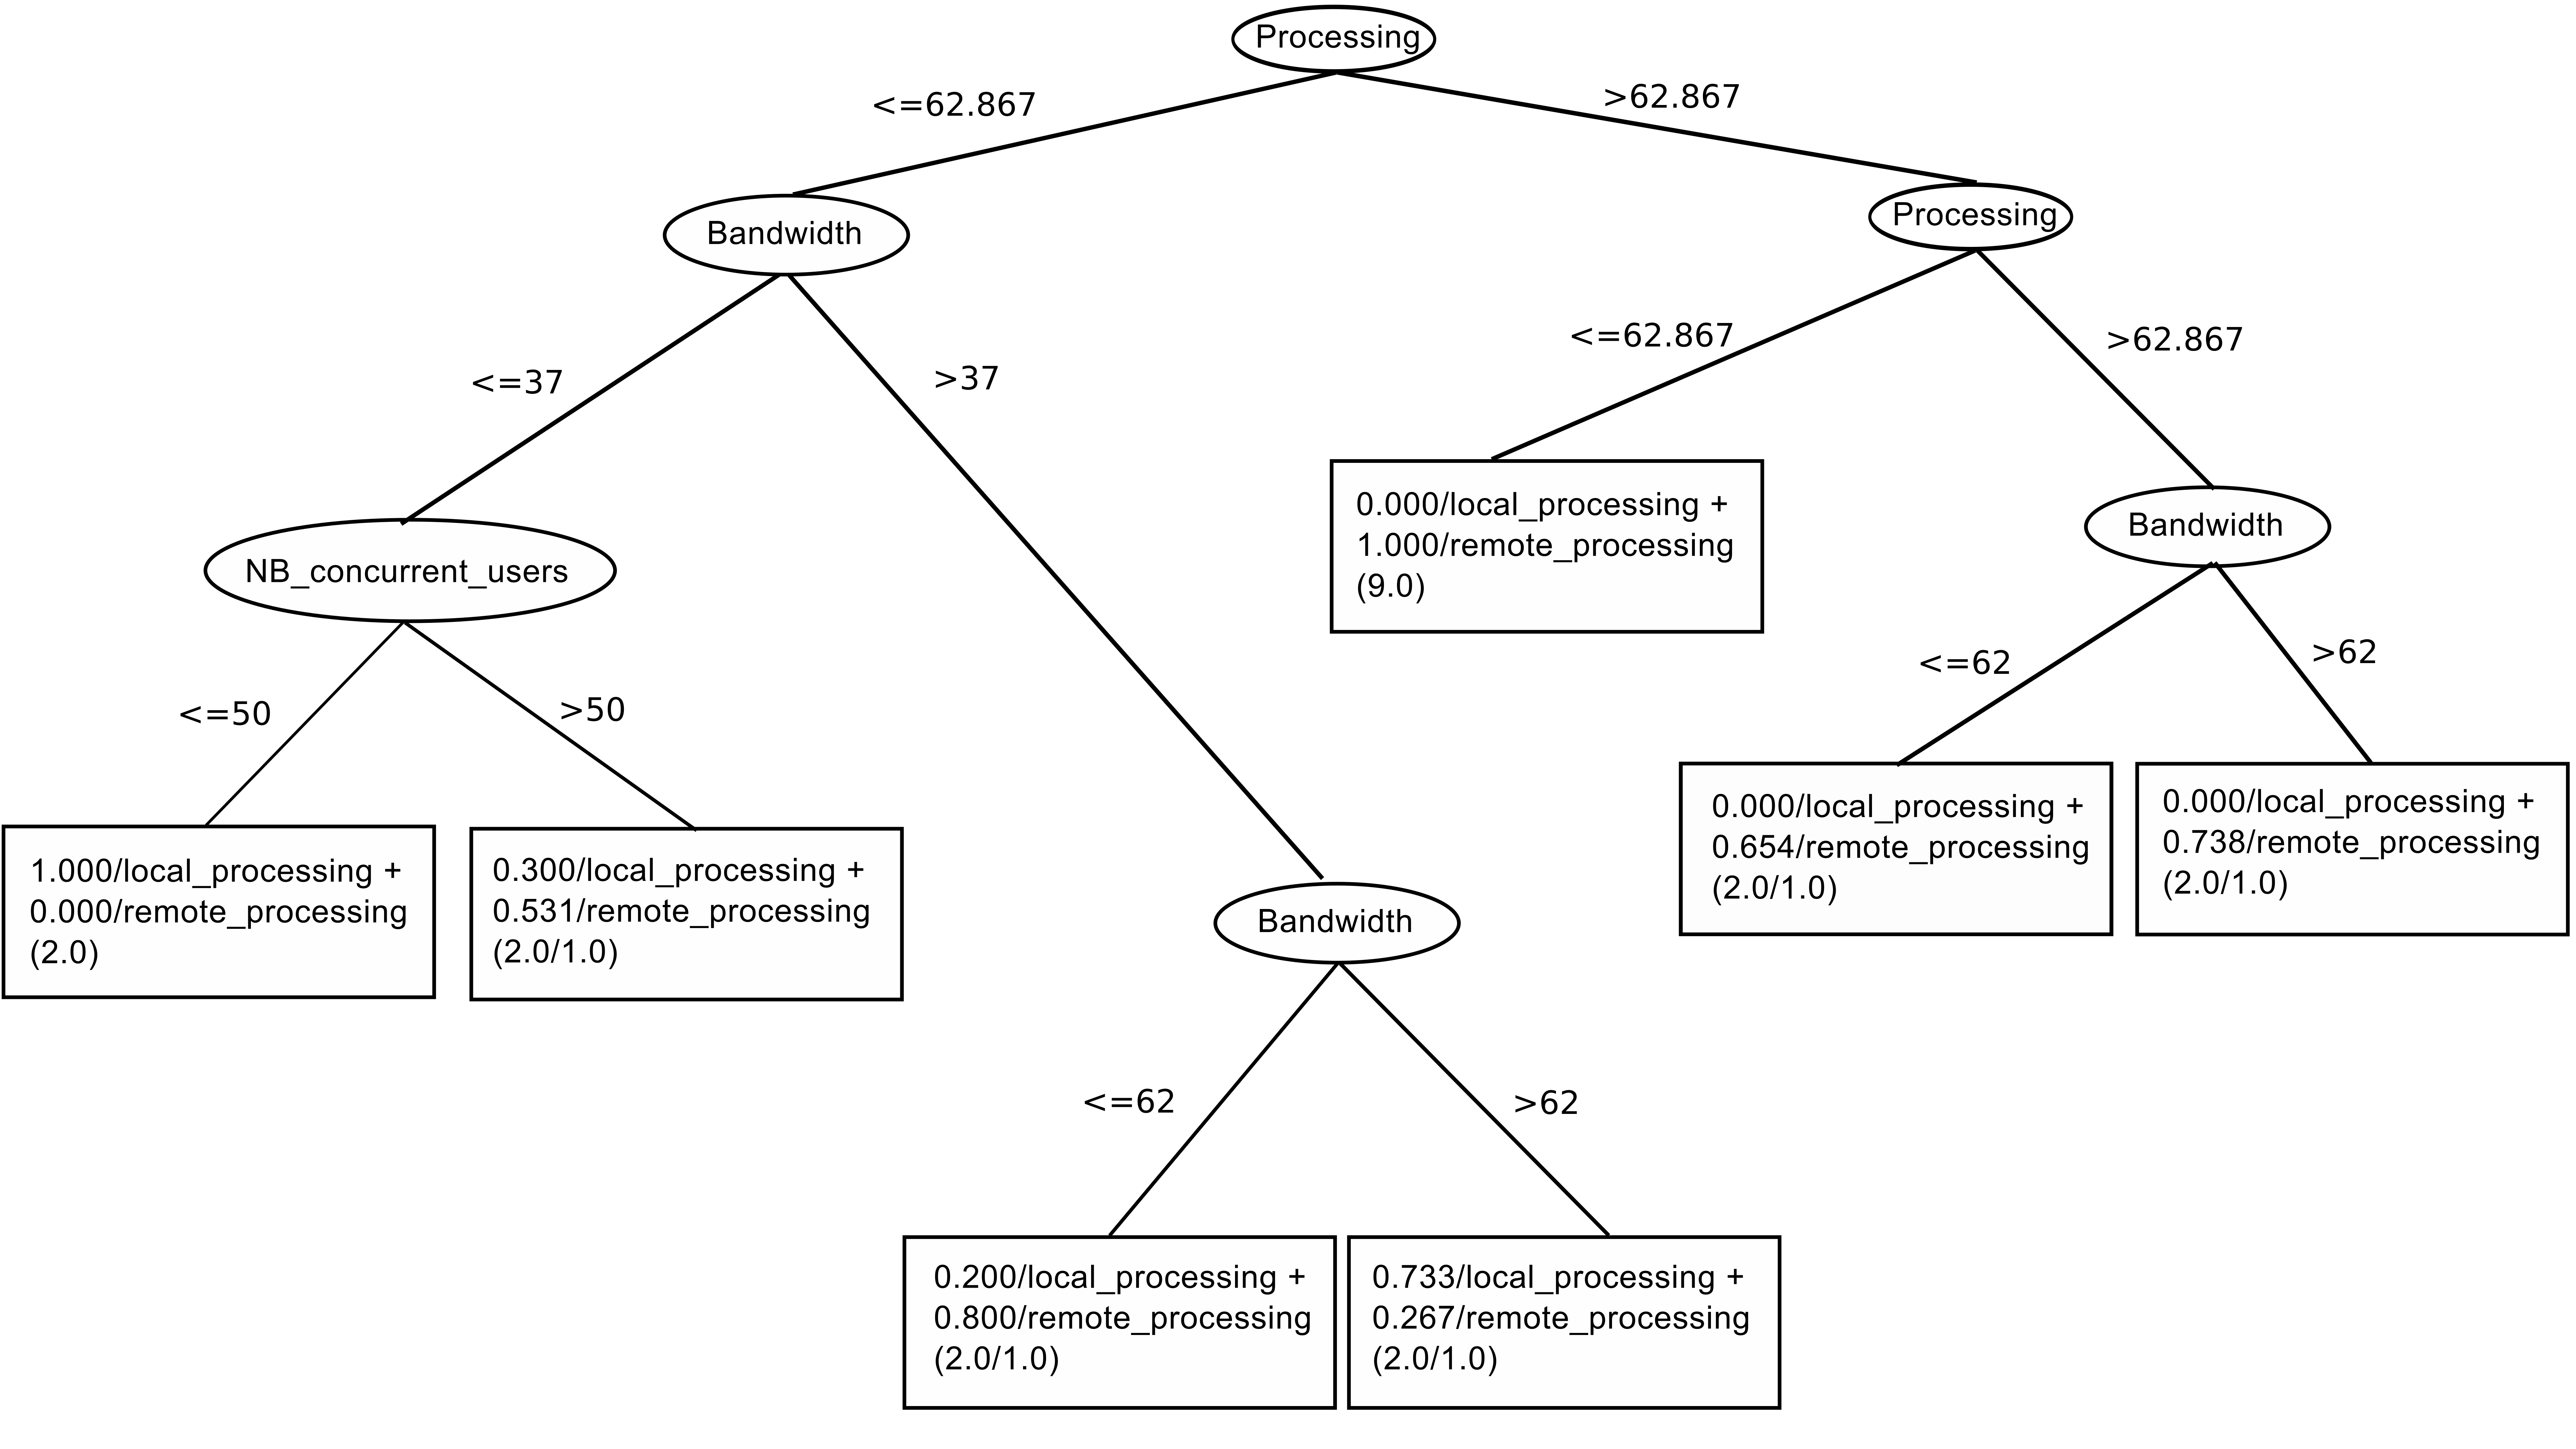
\includegraphics[width=1\textwidth]{../images/decision_tree.png}
  \caption{Decision tree generated by the J48 algorithm. (Recreated with Inkscape)}
  \label{fig:decision-tree}
\end{figure}

\begin{table}[H]
  \centering
  \begin{tabular}{|c|c|c|c|c|}
    \hline
    Name                & Range    & Fuzzy set & Membership function & Parameters    \\
    \hline
    Bandwidth           & [0, 100] & bw_low    & triangular          & 0, 20, 40     \\
    (in Mbps)           &          & bw_med    & triangular          & 35, 37, 70    \\
                        &          & bw_high   & triangular          & 65, 82, 100   \\
    \hline
    Data size           & [0, 600] & data_low  & triangular          & 0, 180, 360   \\
    (in KB)             &          & data_med  & triangular          & 250, 420, 590 \\
                        &          & data_high & triangular          & 450, 600, 600 \\
    \hline
    Load                & [0, 100] & load_low  & triangular          & 0, 20, 40     \\
    (in \%)             &          & load_med  & triangular          & 35, 52, 70    \\
                        &          & load_high & triangular          & 65, 82, 100   \\
    \hline
    Memory              & [0, 100] & mem_low   & triangular          & 0, 20, 40     \\
    (in \%)             &          & mem_med   & triangular          & 35, 52, 70    \\
                        &          & mem_high  & triangular          & 65, 82, 100   \\
    \hline
    Number              & [0, 100] & user_low  & triangular          & 0, 20, 40     \\
    of concurrent users &          & user_med  & triangular          & 30, 50, 70    \\
                        &          & user_high & triangular          & 60, 80, 100   \\
    \hline
  \end{tabular}
  \caption{Input variables for the fuzzy engine.}
  \label{tab:new-fuzzy-input}
\end{table}

\begin{table}[H]
  \centering
  \begin{tabular}{|c|c|c|c|c|}
    \hline
    Name                & Range    & Fuzzy set & Membership function & Parameters      \\
    \hline
    Offloading decision & [0, 100] & local     & triangular          & 0, 24, 48       \\
                        &          & remote    & triangular          & 36, 62.867, 100 \\
    \hline
  \end{tabular}
  \caption{Output variable for the fuzzy engine.}
  \label{tab:new-fuzzy-output}
\end{table}

When defining the membership functions, we usually want them to be symmetrical but in this case, we decided to keep the
values as they were in the decision tree. This resulted in \textbf{Bandwidth} and \textbf{Processing} not having
symmetrical membership functions, \textbf{Data size} is also in this case but for a different reason and is not as
noticeable. We can use the graphic interface of QtFuzzyLite to visualize the new membership functions and compare them
to the original ones. The results are shown in figures \ref{fig:old-fuzzy-engine-inputs}, \ref{fig:old-fuzzy-engine-output},
\ref{fig:new-fuzzy-engine-inputs} and \ref{fig:new-fuzzy-engine-output}.

\subsection{Generating new results with the updated fuzzy engine}
\label{subsec:new-fuzzy-results}

After updating the fuzzy engine, we made a script capable of running both the old and new fuzzy engines with the same
input data. We then compared the results to see if the decision tree improved the accuracy of the fuzzy engine. The
results are shown in tables \ref{tab:old-fuzzy-results} and \ref{tab:new-fuzzy-results}.

\begin{table}[H]
  \centering
  \resizebox{\textwidth}{!}{%
    \begin{tabular}{|l|l|l|l|l|l|l|l|l|}
      \hline
      Bandwidth & Data size & Number of        & Memory & Load & Crisp  & Fuzzy output                                     \\
                &           & concurrent users &        &      & output &                                                  \\
      \hline
      43        & 505       & 44               & 92     & 69   & 67.228 & 0.000/local_processing + 1.000/remote_processing \\
      20        & 285       & 87               & 35     & 93   & 21.6   & 1.000/local_processing + 0.000/remote_processing \\
      83        & 193       & 71               & 71     & 36   & 56.42  & 0.267/local_processing + 0.733/remote_processing \\
      45        & 353       & 9                & 77     & 72   & 67.251 & 0.000/local_processing + 0.946/remote_processing \\
      70        & 61        & 93               & 64     & 17   & 21.6   & 1.000/local_processing + 0.000/remote_processing \\
      28        & 418       & 60               & 35     & 22   & 21.6   & 1.000/local_processing + 0.000/remote_processing \\
      60        & 345       & 31               & 53     & 15   & 62.239 & 0.115/local_processing + 0.885/remote_processing \\
      37        & 400       & 77               & 71     & 18   & 55.221 & 0.300/local_processing + 0.700/remote_processing \\
      \hline
    \end{tabular}}
  \caption{Sample results from the old fuzzy engine.}
  \label{tab:old-fuzzy-results}

  \bigskip

  \centering
  \resizebox{\textwidth}{!}{%
    \begin{tabular}{|l|l|l|l|l|l|l|l|l|}
      \hline
      Bandwidth & Data size & Number of        & Memory & Load & Crisp  & Fuzzy output                                     \\
                &           & concurrent users &        &      & output &                                                  \\
      \hline
      43        & 505       & 44               & 92     & 69   & 66.289 & 0.000/local_processing + 1.000/remote_processing \\
      20        & 285       & 87               & 35     & 93   & 24.0   & 1.000/local_processing + 0.000/remote_processing \\
      83        & 193       & 71               & 71     & 36   & 57.64  & 0.200/local_processing + 0.800/remote_processing \\
      45        & 353       & 9                & 77     & 72   & 66.294 & 0.000/local_processing + 0.961/remote_processing \\
      70        & 61        & 93               & 64     & 17   & 53.206 & 0.339/local_processing + 0.661/remote_processing \\
      28        & 418       & 60               & 35     & 22   & 45.829 & 0.600/local_processing + 0.400/remote_processing \\
      60        & 345       & 31               & 53     & 15   & 62.223 & 0.083/local_processing + 0.917/remote_processing \\
      37        & 400       & 77               & 71     & 18   & 59.483 & 0.150/local_processing + 0.850/remote_processing \\
      \hline
    \end{tabular}}
  \caption{Sample results from the new fuzzy engine.}
  \label{tab:new-fuzzy-results}
\end{table}

We can see that, while some results are nearly identical, others are quite different. The new engine either reinforced the
decision made by the old engine or changed it. Overall, the new engine seems to yield better and more consistent results.
This is worth expending upon in the future by using more data and refining the decision tree. However, we lack the time to
do so in the context of this project.

\begin{figure}[H]
  \centering
  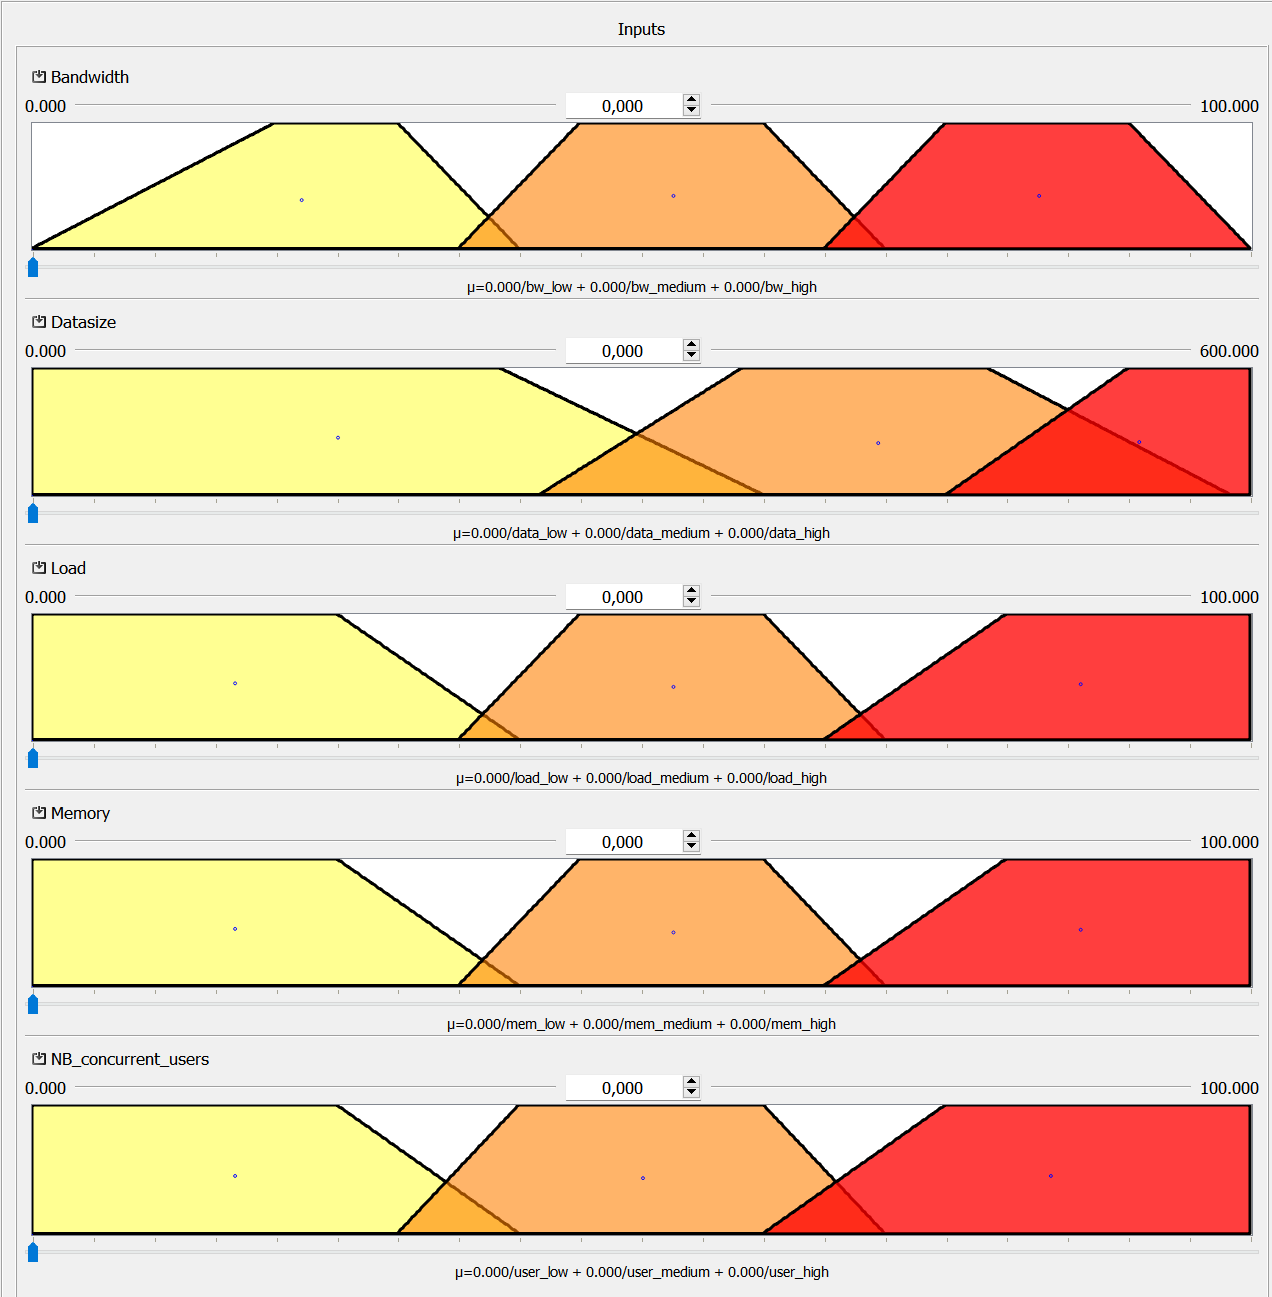
\includegraphics[width=0.63\textwidth]{../images/old-vars-inputs.png}
  \caption{Input variables for the old fuzzy engine.}
  \label{fig:old-fuzzy-engine-inputs}
\end{figure}

\begin{figure}[H]
  \centering
  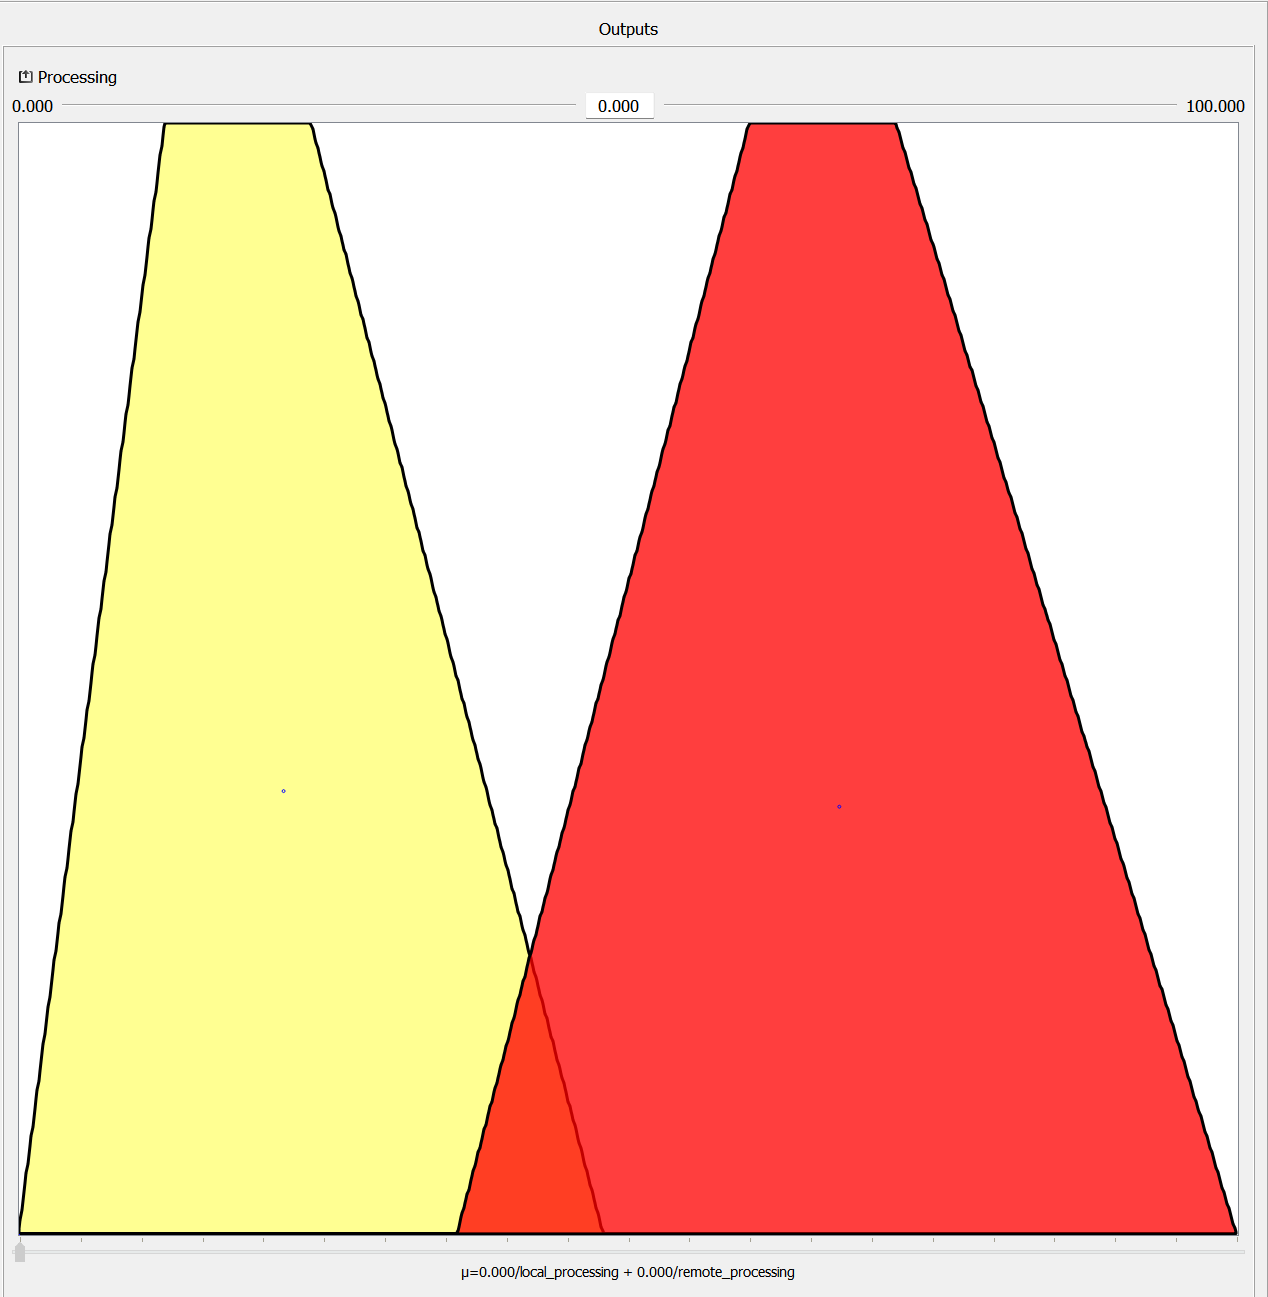
\includegraphics[width=0.63\textwidth]{../images/old-vars-output.png}
  \caption{Output variable for the old fuzzy engine.}
  \label{fig:old-fuzzy-engine-output}
\end{figure}

\begin{figure}[H]
  \centering
  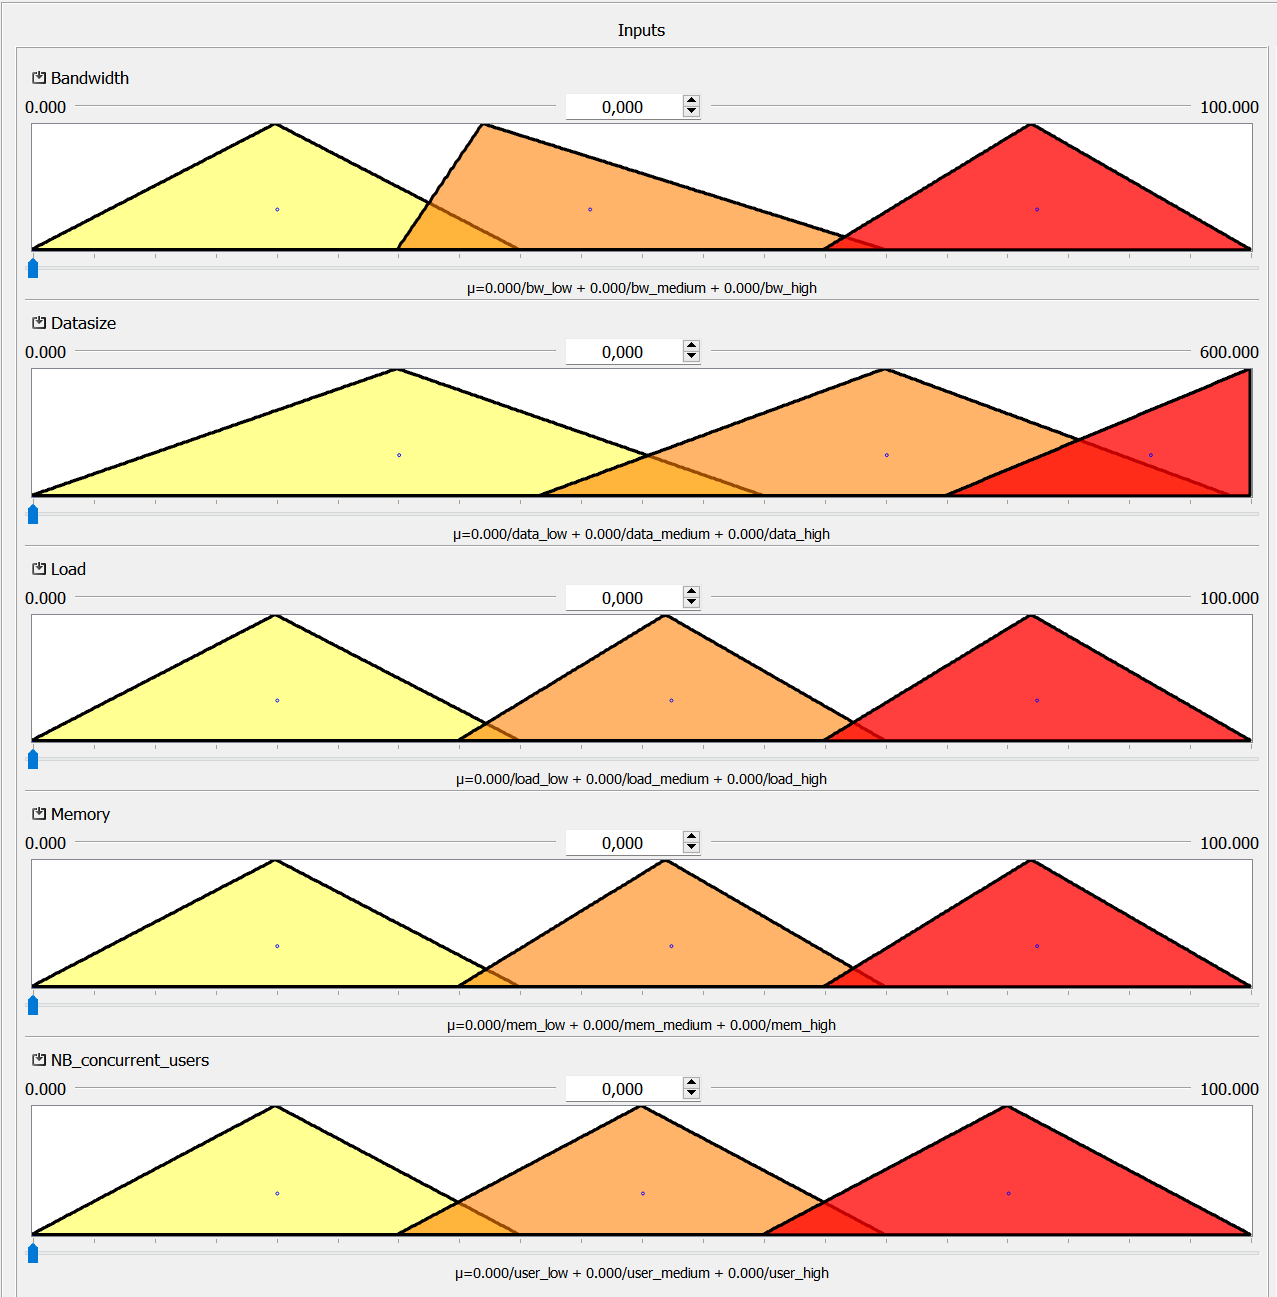
\includegraphics[width=0.63\textwidth]{../images/new-vars-inputs.png}
  \caption{Input variables for the new fuzzy engine.}
  \label{fig:new-fuzzy-engine-inputs}
\end{figure}

\begin{figure}[H]
  \centering
  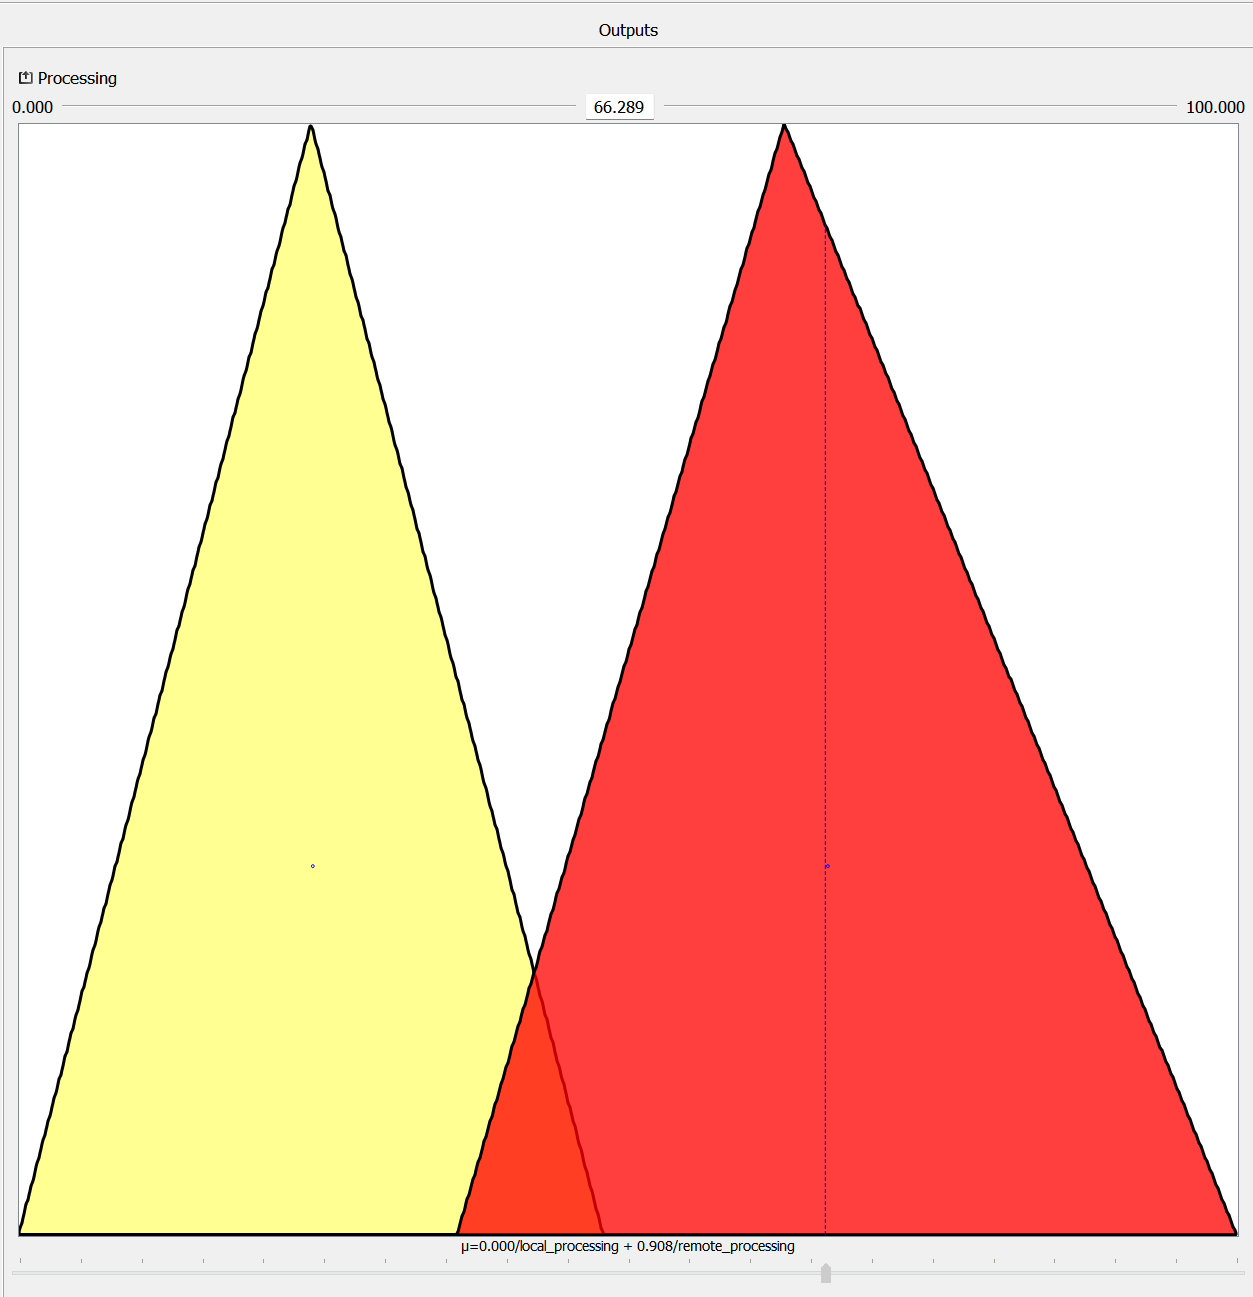
\includegraphics[width=0.63\textwidth]{../images/new-vars-output.png}
  \caption{Output variable for the new fuzzy engine.}
  \label{fig:new-fuzzy-engine-output}
\end{figure}
